\section{Introduzione}

\subsection{Glossario}
In questo documento sono state segnate con il pedice "g" tutte le parole che, secondo noi, necessitano di una spiegazione ulteriore per evitare
eventuali ambiguità o incomprensioni.

La spiegazione di questi termini la si può trovare nel documento di \textit{Glossario}.

\subsection{Scopo del documento}
Il documento \textit{Specifica Tecnica} ha lo scopo di descrivere i componenti utilizzati e le scelte progettuali fatte per la realizzazione del prodotto.

Dopo aver fornito un elenco descrittivo dei componenti verranno spiegati nel dettaglio, utilizzando l'ausilio degli schemi UML, i seguenti punti di interesse: 
\begin{itemize}
	\item Design pattern architetturale determinato dalle tecnologie adottate;
	\item Architettura logica (connessioni e interazioni tra componenti);
	\item Architettura di deployment (l’allocazione di componenti nel sistema in esecuzione);
	\item Idiomi, pattern di livello più basso che architetturale;
	\item Ogni altro aspetto progettuale che valorizza o caratterizza il design utilizzato.
\end{itemize}

\subsection{Suggerimenti per la comprensione del documento}
Per comprendere al meglio l'architettura utilizzata è importante comprendere in primo luogo il design pattern
architetturale derterminato dalle tecnologie adottate in quanto gran parte delle scelte fatte si basano su di esso.

\textbf{Si suggerisce quindi di leggere la sezione} \ref{design Redux} \textbf{riguardante il design pattern architetturale determinato 
dalle tecnologie adottate prima di proseguire con le successive}.

\subsection{Riferimenti}
\subsubsection{Riferimenti normativi}
\begin{itemize}
\item .
\end{itemize}

\subsubsection{Riferimenti informativi}
\begin{itemize}
\item .
\end{itemize} 

\section{Descrizione dell'architettura}
\subsection{Elenco dei componenti}
\begin{itemize}
	\item \textbf{\large Slices}:
		\begin{itemize}
			\item \textbf{CartSlice}: componente che permette la gestione dello stato che contiene i dati riguardanti il carrello;
			\item \textbf{ProductsSlice}: componente che permette la gestione dello stato che contiene i dati riguardanti i prodotti 
			presenti all'interno dell'ambiente 3D;
			\item \textbf{PlayerSlice}: componente che permette la gestione dello stato che contiene i dati riguardanti il player;
			\item \textbf{RayCasterSlice}: componente che permette la gestione dello stato che contiene i dati riguardanti il
			prodotto con cui è possibile interagire nell'ambiente 3D;
			\item \textbf{DecorationSlice}: componente che permette la gestione dello stato che contiene i dati riguardanti
			il caricamento delle decorazioni all'interno dell'ambiente 3D;
			\item \textbf{SidebarSlice}: componente che permette la gestione dello stato che contiene i dati riguardanti
			la side-bar;
		\end{itemize}
	\item \textbf{\large Initial states}:
	Gli stati iniziali contengono i dati di interesse comune tra componenti in modo da facilitarne il reperimento.
	I dati che non sono di iteresse comune risiedono internamente ai componenti che li utilizzano.
		\begin{itemize}
			\item \textbf{CartInitialState}: componente che contiene i dati relativi agli oggetti presenti all'interno del carrello;
			\item \textbf{ProductsInitialState}: componente che contiene i dati relativi ai prodotti presenti all'interno dell'ambiente 3D;
			\item \textbf{PlayerInitialState}: componente che contiene i dati relativi al player;
			\item \textbf{RayCasterInitialState}: componente che contiene i dati utili ad interagire con un oggetto presente all'interno dell'
			ambiente 3D;
			\item \textbf{DecorationInitialState}: componente che contiene la lista di tutte le decorazioni presenti all'interno dell'ambiente 3D;
			\item \textbf{SidebarInitialState}: componente che contiene i dati utili a reperire informazioni sulla sidebar;
		\end{itemize}
		\item \textbf{\large Actions}:
		Per convenzione il nome delle azioni seguono il formato: [nome Slice dalla quale viene catturata].[nome azione]
		\begin{itemize}
			\item \textbf{sidebar.toggleSidebarIsOpen}: azione emessa quando si apre o si chiude la sidebar relativa ad un prodotto presente 
			all'interno della scena 3D.
			\\
			Payload: nessuno;
			\item \textbf{sidebar.setSelectedColor}: azione emessa quando si seleziona nella sidebar un nuovo colore per un prodotto.
			\\
			Payload: \{id:number, selectedColor: String\};
			\\
			id: ID del prodotto a cui cambiare il colore.
			\\
			selectedColor: colore selezionato;
			\item \textbf{rayCaster.setLastProductPointed}: azione emessa per aggiornare l'ID che rappresenta l'ultimo oggetto puntato dal raycaster.
			\\
			\textit{Payload}: \{id:number\}
			\\
			id: ID dell'ultimo prodotto puntato dal raycaster;
			\item \textbf{rayCaster.toggleRayCasterEnabled}: azione emessa per abilitare o disabilitare il raycaster.
			\\
			\textit{Payload}: nessuno;
			\item \textbf{cart.addItems}: azione emessa per aggiungere uno o più prodotti al carrello.
			\\
			\textit{Payload}: {id: number, price: number, quantity: number,selectedColor: String}
			\\
			id: ID del prodotto da aggiungere al carrello.
			\\
			price: prezzo del prodotto da aggiungere al carrello.
			\\
			quantity: quantità di prodotti da aggiungere al carrello.
			\\
			selectedColor: colore selezionato del prodotto da aggiungere al carrello.
			\item \textbf{cart.removeItem}: azione emessa per rimuovere un prodotto dal carrello.
			\\
			Payload: nessuno;
			\item \textbf{cart.removeAll}: azione emessa per rimuovere tutti i prodotti presenti nel carrello.
			\\
			Payload: nessuno;
		\end{itemize}
		\item \textbf{\large Model components}:
		\begin{itemize}
			\item \textbf{Coordinate}: classe 
			\item \textbf{Camera}: classe offerta dalla libreria three.js.
			Rappresenta l'utente all'interno dell'ambiente 3D.
			Modificando gli attributi di questa classe l'utente compie movimenti spaziali e può esplorare l'ambiente che 
			lo circonda da prospettive diverse.
			\item \textbf{Octree}: classe offerta dalla libreria three.js.
			L'Octree è una struttura dati ad albero utilizzata per la rappresentazione e la gestione di dati spaziali 
			tridimensionali. 
			In particolare, viene utilizzata per dividere lo spazio tridimensionale in regioni più piccole, 
			suddividendo ciascuna regione in otto sotto-regioni.
			Utile per determinare con quale prodotto si sta interagendo o per rilevare le collisioni.
			\item \textbf{Vector3}: classe offerta dalla libreria three.js.
			Rappresenta un vettore tridimensionale, ovvero una grandezza fisica caratterizzata da una direzione e da una lunghezza.
			Il vettore tridimensionale viene comunemente utilizzato per definire la posizione, la rotazione, 
			la scala e la direzione degli oggetti all'interno di una scena 3D. 
			\item \textbf{Capsule}: classe offerta dalla libreria three.js.
			La classe Capsule offre la possibilità di impostare una forma di collisione personalizzata 
			per l'oggetto rappresentato dalla capsula. 
			\item \textbf{Player}: classe con il compito di tenere traccia ed aggiornare le informazioni riguardanti 
			lo stato dell'utente all'interno dell'ambiente 3D.
			Le informazioni principali di cui si occupa la classe sono la posizione spaziale, la posizione della camera,
			la velocità dell'utente o se l' utente si trova in una posizione sopraelevata rispetto al piano che rappresenta 
			lo zero della scena.
			\item \textbf{CartItem}: classe che rappresenta un item all'interno del carrello.
			Quando viene aggiunto un prodotto al carrello viene creato un item che ne raccoglie le informazioni utili 
			alla sua visualizzazione all' interno del carrello e all'acquisto.
		\end{itemize}
		\item \textbf{\large UI React components}:
		I seguenti componenti hanno il compito di visualizzare i dati del modello e costituiscono l'interfaccia 
		utente. 
		\begin{itemize}
			\item \textbf{UI}: componente React che contiene i componenti grafici che vanno a costituire l'interfaccia
			utente. 
			\item \textbf{Crosshair}: componente react-three-fiber che viene utilizzato per aiutare l'utente a puntare
			un determinato punto nello spazio 3D.
			Solitamente viene indicato con un punto o una croce al centro dello schermo ed usato come puntatore dall'utente.
			\item \textbf{Cart}: componente React che rappresenta il carrello.
			\item \textbf{PlayerPosition}: componente React con il compito di visualizzare a schermo la posizione in cui 
			si trova l'utente all'interno della scena 3D.
			\item \textbf{CartItem}: componente React che rappresenta un prodotto all'interno del carrello.
			Contiene le informazioni basilari necessarie alla visualizzazione e all'acquisto di un prodotto.
			\item \textbf{ProductUI}:  componente React che contiene i componenti dell'interfaccia utente per la visualizzazione
			del ProductInteractionPrompt e della sidebar.
			\item \textbf{ProductInteractionPrompt}: componente React che contiene i componenti grafici che vanno a costituire 
			la parte dell'interfaccia utente relativa alla visualizzazione del nome del prodotto con cui si sta interagendo.
			\item \textbf{Sidebar}: componente React che contiene i componenti necessari a visualizzare i 
			dettagli del prodotto con cui si sta iteragendo e i componenti con cui è possibile modificare le caratteristiche del 
			prodotto e aggiungerne la quantità specificata al carrello.
			\item \textbf{ColorSelector}: componente React che contiene i componenti necessari per compiere un'azione di selezione colore.
			\item \textbf{SelectColorItem}: componente React con cui è possibile compiere un'azione di selezione colore.
			\item \textbf{ProductDetails}: componente React per la visualizzazione dei dettagli di un prodotto.
		\end{itemize}
		\item \textbf{\large 3D React components}:
		I seguenti componenti hanno il compito di visualizzare i dati del modello costituiscono il canvas 
		sul quale viene renderizzata la scena 3D.
		\begin{itemize}
			\item \textbf{Canvas}: componente react-three-fiber che comprende gli elementi grafici che vanno a costituire
			la scena 3D.
			Il componente Canvas si occupa di creare un nuovo canvas HTML e di associarlo a una nuova istanza di THREE.WebGLRenderer, 
			che viene utilizzata per renderizzare la scena Three.js all'interno del componente React.
			Fornisce una camera e una serie di props opzionali utili alla configurazione dell'ambiente 3D.
			\item \textbf{Scene}: componente react-three-fiber che rappresente l'ambiente 3D.
			Si tratta di uno spazio virtuale 3D in cui gli oggetti vengono posizionati, orientati e illuminati.
			\item \textbf{PointerLock}: componente react-three-fiber che consente di fare le richieste di PointerLock fornite da
			three.js. 
			Un pointerLock consente di controllare la camera e di disattivare i controlli della camera quando 
			necessario (ad esempio quando si apre un menu di interazione con un prodotto).
			\item \textbf{Environment}: componente react-three-fiber utilizzato per creare una scena base configurata
			secondo impostazioni standard settabili.
			\item \textbf{Map}: componente React che contiene i componenti che costituiscono la scena.
			Tra essi possiamo trovare: player, lights, models, decorations, raycaster.
			\item \textbf{Player}: componente React che contiene il player.
			\item \textbf{Lights}: componente React che rappresenta le luci all'interno della scena.
			\item \textbf{Models}: componente React che rappresenta un prodotto all'interno dell'ambiente 3D.
			I modelli vengono caricati all'interno della scena specificandonone il path del modello .gltf, la posizione
			in cui si vogliono collocare e le caratteristiche del prodotto legato al modello da caricare.
			\item \textbf{Decorations}: una decorazione è un modello .gltf che si differisce dal modello di un prodotto 
			per il fatto che non è modificabile e non può essere aggiunto al carrello.
			\item \textbf{RayCaster}: componente three.js che rappresenta un oggetto utilizzato per effettuare 
			collisioni e interazioni tra gli oggetti nella scena e il puntatore del mouse.
			Il raycaster genera un raggio virtuale che parte dalla posizione del puntatore del mouse e attraversa lo schermo fino a 
			raggiungere un oggetto nella scena, se presente. 
			È possibile quindi utilizzare questa informazione per eseguire azioni in risposta all'interazione dell'utente.
		\end{itemize}
\end{itemize}
\subsection{Design pattern architetturale determinato dalle tecnologie adottate}
\label{design Redux}

\subsubsection{Redux-Toolkit}
I componenti che costituiscono l'architettura utilizzata seguono il pattern offerto dalla libreria Redux-Toolkit.

Redux-Toolkit è pensato per integrarsi con React e il principale vantaggio che offre è quello di poter gestire i dati condivisi tra 
i componenti React in modo centralizzato semplificando la gestione dello stato globale dell'applicazione 
(in alternativa ogni componente React dovrebbe passare il proprio stato tramite props ai suoi diretti discendenti).
\\\\
I componenti che formano l'architettura di Redux-Toolkit sono:
\begin{itemize}
	\item \textbf{Store}: componente che contiene lo stato globale dell'applicazione.
	
	All'avvio dell'applicazione viene configurato utilizzando RootReducer e i componenti che utilizzano lo stato globale fanno il subscribe allo \textit{store}
	in modo da venire renderizzati ogni volta che un dato di interesse cambia valore.
	Questo modo di operare può essere visto come un pattern \textit{Observer} in cui lo \textit{store} è il \textit{Subject} e gli \textit{Observers} sono i componenti React che hanno fatto 
	il subscribe allo \textit{store};
	\item \textbf{RootReducer}: componente utilizzato per configurare lo store combinando più slice;
	\item \textbf{Slice}: componente che contiene un proprio stato che rappresenta una porzione dello stato globale dell'applicazione, i \textit{reducer}
	che operano sullo stato e i \textit{selector} per consentire ai suoi client il reperimento dei dati. 

	Per definire una \textit{slice} è buona norma raggruppare i dati in modo che siano legati da un sottoinsieme di funzionalità offerte dal sistema che lavorano 
	su dati comuni;  
	\item \textbf{Reducer}: componente che riceve come parametri uno stato iniziale (\textit{InitialState}) e una \textit{action} (composta da un type e un payload) e restituisce 
	lo stato dopo aver operato sui dati. 
	
	React-Toolkit gestisce le chiamate ai \textit{reducer} quindi i dispatch delle \textit{action} avvengono
	specificando solamente l'oggetto che rappresenta il payload; 
	\item \textbf{Actions}: oggetto composto da un type e da un payload di cui viene effettuato il dispatch quando opportuno. 
	
	Il payload è un oggetto che contiene i dati da passare al \textit{reducer} che catturerà l'\textit{action};
	\item \textbf{InitialState}: componente che contiene i dati di una \textit{slice} su cui essa opera. 
	
	Importante precisare che Redux-Toolkit utilizzando 
	la libreria immer gestisce anche l'immutabilità dei dati in modo che i reducer restituiscano delle copie dello stato in modo che esso non possa 
	venire modificato dall'esterno e utilizzato in modo improrio.
	
	L'unico modo per modificare i dati dello stato globale è quindi con il dispatch di un'\textit{action};
	\item \textbf{Selector}: funzione che prende lo stato corrente di una \textit{slice} come argomento e ritorna un sottoinsieme specifico
	del suo stato. In altre parole, un \textit{selector} consente di 'selezionare' una parte specifica dello stato
	in modo da poterla utilizzare in modo isolato all'interno di un componente React.
\end{itemize}

\subsubsection{React-three-fiber}
Questa libreria fornisce un 'punto d'incontro' tra React (libreria javascript per la creazione di interfacce utente) e Three.js (libreria usata per
la modellazione dell'ambiente 3D) semplificando la creazione dei componenti da inserire all'interno dell'ambiente 3D.

React-three-fiber rende la scrittura del codice dichiarativa creando dei componenti React 'preconfezionati' che rappresentano i componenti 3D.
Questi componenti sono personalizzabili modificandone le caratteristiche tramite le props di React.

Un esempio è il componente \textit{Canvas} che fornisce con un'unica dichiarazione la \textit{scene} e la \textit{camera} con una configurazione standard 
adatta alla maggior parte dei casi di utilizzo. Per inserire i componenti all'interno dell'ambiente è sufficiente dichiararli come figli del 
componente \textit{scene}.
\subsection{Architettura logica}
Per facilitare la lettura dei diagrammi delle classi è stato scelto di organizzarli per feature in modo che ogni diagramma 
rappresenti i componenti che permettono l'implementazione di funzionalita' specifiche.
Sono presenti dei diagrammi che non seguono questa convenzione che sono utili per avere una visione generale sulle dipendenze
di alcuni componenti.
\\\\
I diagrammi prodotti che rappresentano funzionalità specifiche sono:
\begin{itemize}
	\item \textbf{CartFeaturesDiagram:} include i componenti che svolgono le funzioni riguardanti il carrello;
	\item \textbf{PlayerFeaturesDiagram:} include i componenti che svolgono le funzioni riguardanti le interazioni dell'utente con 
	l'ambiente 3D;
	\item \textbf{ProductSidebarFeaturesDiagram:} include i componenti che svolgono le funzioni riguardanti la side-bar;
	\item \textbf{InterfaceFeaturesDiagram:} include i componenti necessari per il corretto aggiornamento dell'interfaccia utente;
\end{itemize}
I diagrammi prodotti che forniscono una visione generale delle dipendenze tra componenti sono:
\begin{itemize}
	\item \textbf{StoreDiagram:} include lo \textit{store};
	\item \textbf{ReactComponentsHierarchy:} include i componenti React che rappresentano l'interfaccia utente e la scena 3D.
\end{itemize}

\subsubsection{CartFeaturesDiagram}
\label{CartFeaturesDiagram}
\begin{figure}[H]
	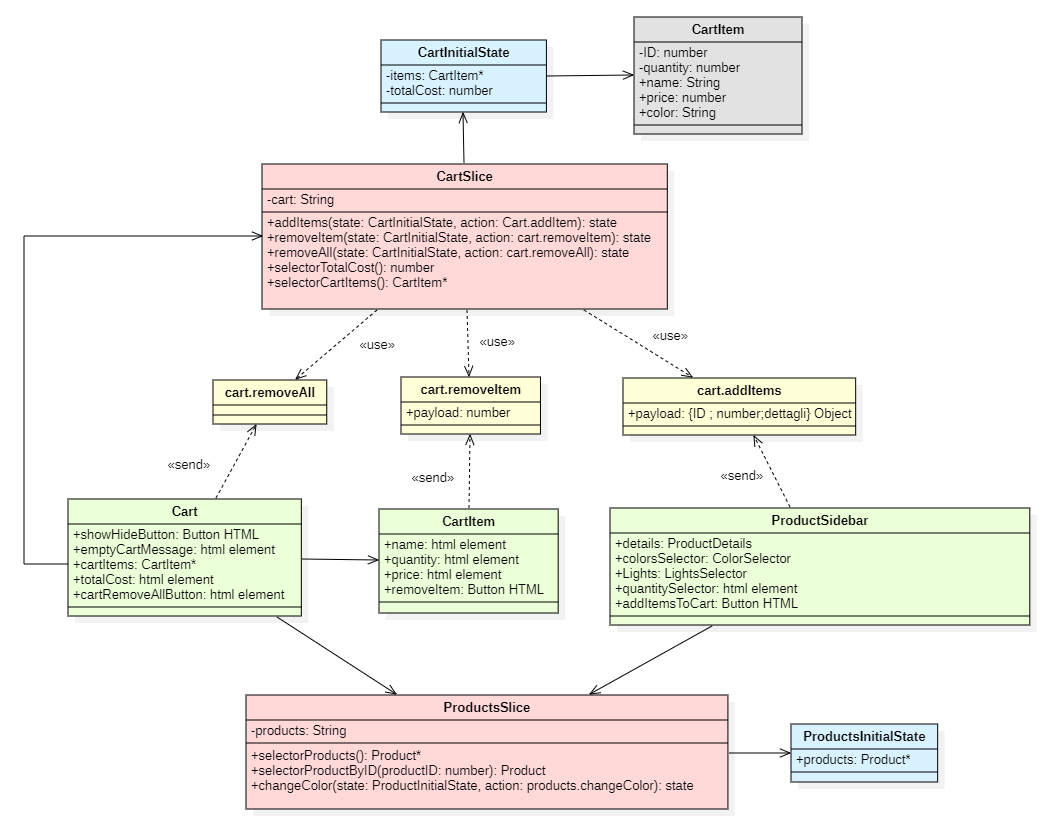
\includegraphics[width=1\textwidth, keepaspectratio]{./res/images/cart_features.PNG}
	\caption[UML delle classi CartFeaturesDiagram]{
	UML delle classi CartFeaturesDiagram.
	\\
	\textbf{Legenda}: 
	[\textit{Slices}: rosso] -
	[\textit{Actions}: giallo] -
	[\textit{Model classes}: grigio] -
	[\textit{Initial states}: azzurro] -
	[\textit{UI React components}: verde]}
\end{figure}

\paragraph*{Descrizione del diagramma:}
CartFeaturesDiagram contiene i componenti coinvolti nelle interazioni con il carrello.
\begin{itemize}
		\item \textbf{CartSlice}
		\begin{itemize}
			\item \textit{Connessioni}: 
			\item \textit{Interazioni}:
		\end{itemize}
		\item \textbf{ProductsSlice}
		\begin{itemize}
			\item \textit{Connessioni}:
			\item \textit{Interazioni}:
		\end{itemize} 
		\item \textbf{CartInitialState}
		\begin{itemize}
			\item \textit{Connessioni}:
			\item \textit{Interazioni}:
		\end{itemize} 
		\item \textbf{ProductsInitialState}
		\begin{itemize}
			\item \textit{Connessioni}:
			\item \textit{Interazioni}:
		\end{itemize} 
		\item \textbf{cart.removeAll}
		\begin{itemize}
			\item \textit{Connessioni}:
			\item \textit{Interazioni}:
		\end{itemize} 
		\item \textbf{cart.removeItem}
		\begin{itemize}
			\item \textit{Connessioni}:
			\item \textit{Interazioni}:
		\end{itemize} 
		\item \textbf{cart.addItems}
		\begin{itemize}
			\item \textit{Connessioni}:
			\item \textit{Interazioni}:
		\end{itemize} 	
		\item \textbf{CartItem}
		\begin{itemize}
			\item \textit{Connessioni}:
			\item \textit{Interazioni}:
		\end{itemize} 
		\item \textbf{Cart}
		\begin{itemize}
			\item \textit{Connessioni}:
			\item \textit{Interazioni}:
		\end{itemize} 
		\item \textbf{CartItem}
		\begin{itemize}
			\item \textit{Connessioni}:
			\item \textit{Interazioni}:
		\end{itemize} 
		\item \textbf{ProductSidebar}
		\begin{itemize}
			\item \textit{Connessioni}:
			\item \textit{Interazioni}:
		\end{itemize} 
	\end{itemize}
	


\subsubsection{PlayerFeaturesDiagram}


\subsubsection{SidebarFeaturesDiagram}


\subsubsection{InterfaceFeaturesDiagram}


\subsubsection{StoreDiagram}


\subsection{Architettura di deployment}
\subsection{Idiomi e pattern di livello più basso}
\subsection{Altri aspetti di design}
























